\chapter{Proposed Framework}
As it has shown, one of the main task of Predictive Maintenance is anomaly detection, described as a set of techniques to identify some anomalous warning states in which an under observation machine could be, allowing a better maintenance activities planning. In this part of the work it is firstly formalized the task performed and then the proposed architecture is illustrated. At the end of the work there is a brief explanation of the technologies used for the implementation of the illustrated framework.
\section{Problem definition}
In this section we formalize the performed anomalous sound detection task. The proposed architecture must learn to classify audio clips placed in input as normal or anomalous. The training set is composed by $K$ audio clips $\{x_1, x_2, ...,x_K\}$ in \textit{.wav} format, recorded from different kinds of a particular machine $X$, with a duration of $T$ seconds. A numerical ID, contained into each clip filename, is used to identify the different kinds of $X$. The goal of this problem is to train a model on all clips that belong to $X$ normal working state and, since only few audio clips are recorded when anomalies are present, they are incorporated into a different set, used for testing the model. For these reasons, this task cannot be solved as a simple classification problem, even though it seems to be a two-class classification problem.\\
Before describing the proposed model in detail, let’s have a look to the im- plemented framework in high level way (Figure \ref{high-level-architecture}). As it can be seen, the input consists in an audio clip microphones disposed around the monitored machinery, while the output is a label, \textit{normal} or \textit{anomaly}.
\begin{figure}[ht]
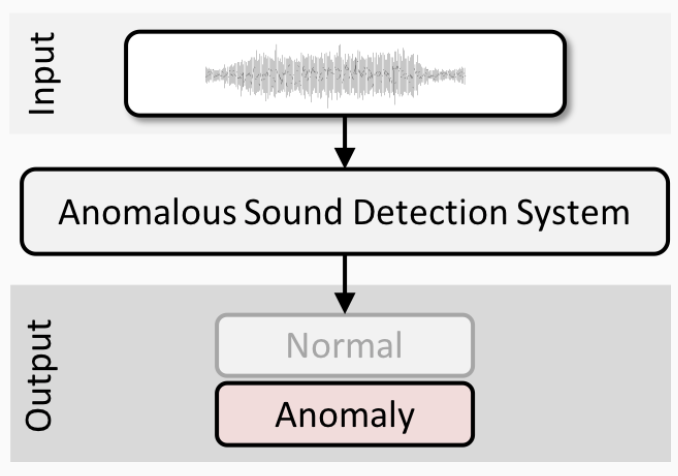
\includegraphics[scale=0.7]{TESI DI FIORE/img/high-level-architecture.png}
\centering
\caption{High level architecture \cite{DCASE}}
\label{high-level-architecture}
\end{figure}

\section{Model architecture}
The proposed ASD system shown in Figures \ref{offline-asd-system} and \ref{online-asd-system} consists of two main phases: an offline training phase responsible of the generation of an autoencoder model and an online operation phase to conduct the ASD in real time. It is good to say immediately that this architecture is valid for every implementation of the autoencoder. In fact, the novelty brought by this work is a generalization of ID embedding idea, shown in Chapter 2 and implemented for DCASE 2020 task 2 Dataset, through the use of different kinds of autoencoders, in terms of how the encoder or the decoder layers are built.\\
In the next two subsections there are a detailed descriptions of the two phases, with a focus on each block present in the pipelines.

\subsection{Offline Training Phase}
\begin{figure}[ht]
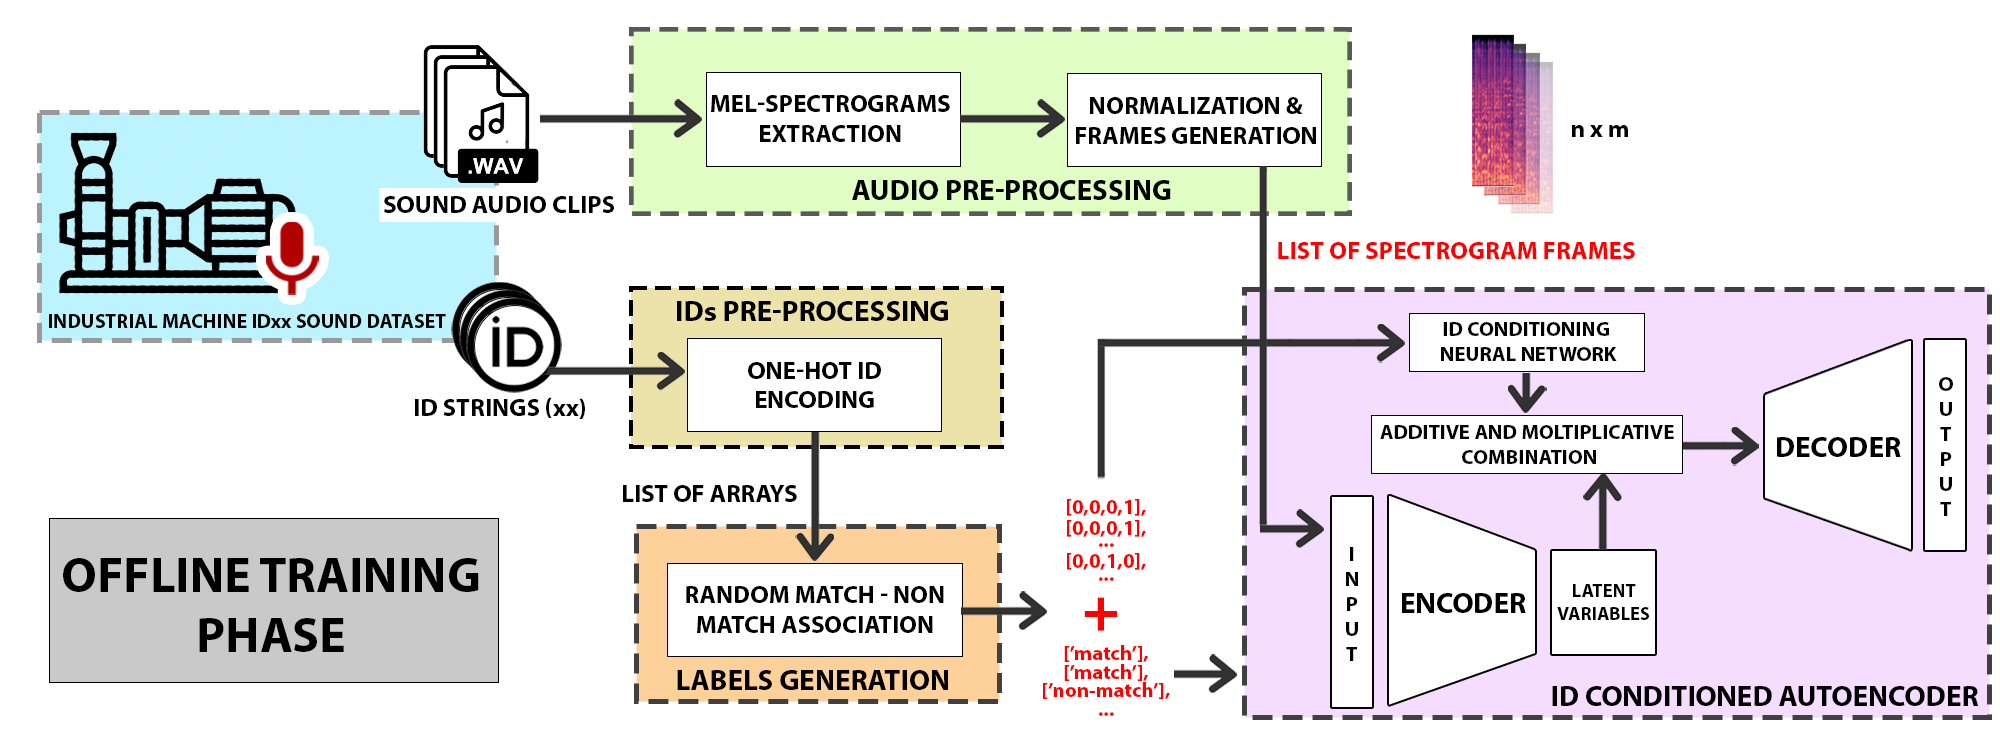
\includegraphics[scale=0.45]{TESI DI FIORE/img/offline-architecture.png}
\centering
\caption{Overview of offline training phase of the proposed ASD system.}
\label{offline-asd-system}
\end{figure}



\subsection{Online Training Phase}
\begin{figure}[ht]
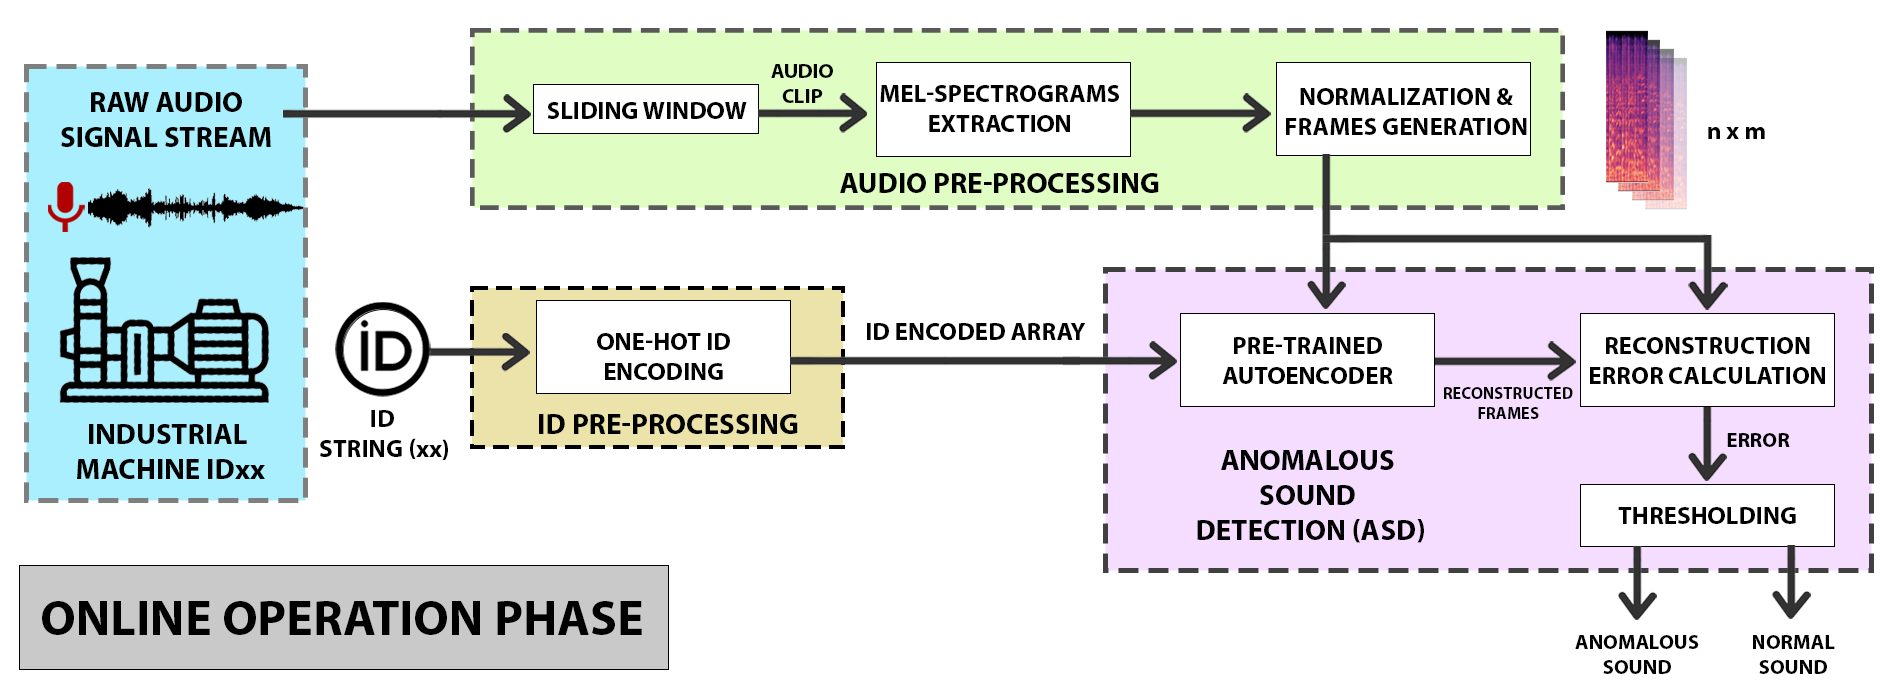
\includegraphics[scale=0.45]{TESI DI FIORE/img/online-architecture.png}
\centering
\caption{Overview of online operating phase of the proposed ASD system.}
\label{online-asd-system}
\end{figure}

\section{Hyperparameters}

\section{Implementation technologies}
In this section, some implementation details about the proposed model are given. The model was implemented in Python 3. Used technologies and libraries are:
\begin{itemize}
    \item {Google Colab: Colab notebooks are Jupyter notebooks that run in the cloud and are highly integrated with Google Drive, making them easy to set up, access, and share;}
    \item {Tensorflow: it is an end-to-end open source platform for Machine Learning;}
    \item {Keras: it is an open source Deep Learning API written in Python3;}
    \item {NumPy, used to work in an efficient way with arrays;}
    \item {SciKit-Learn, a machine learning library, containing simple and efficient tools for predictive data analysis}
\end{itemize}

